\subsection{Structure and mechanics}

EMPTY

\begin{figure}[h]
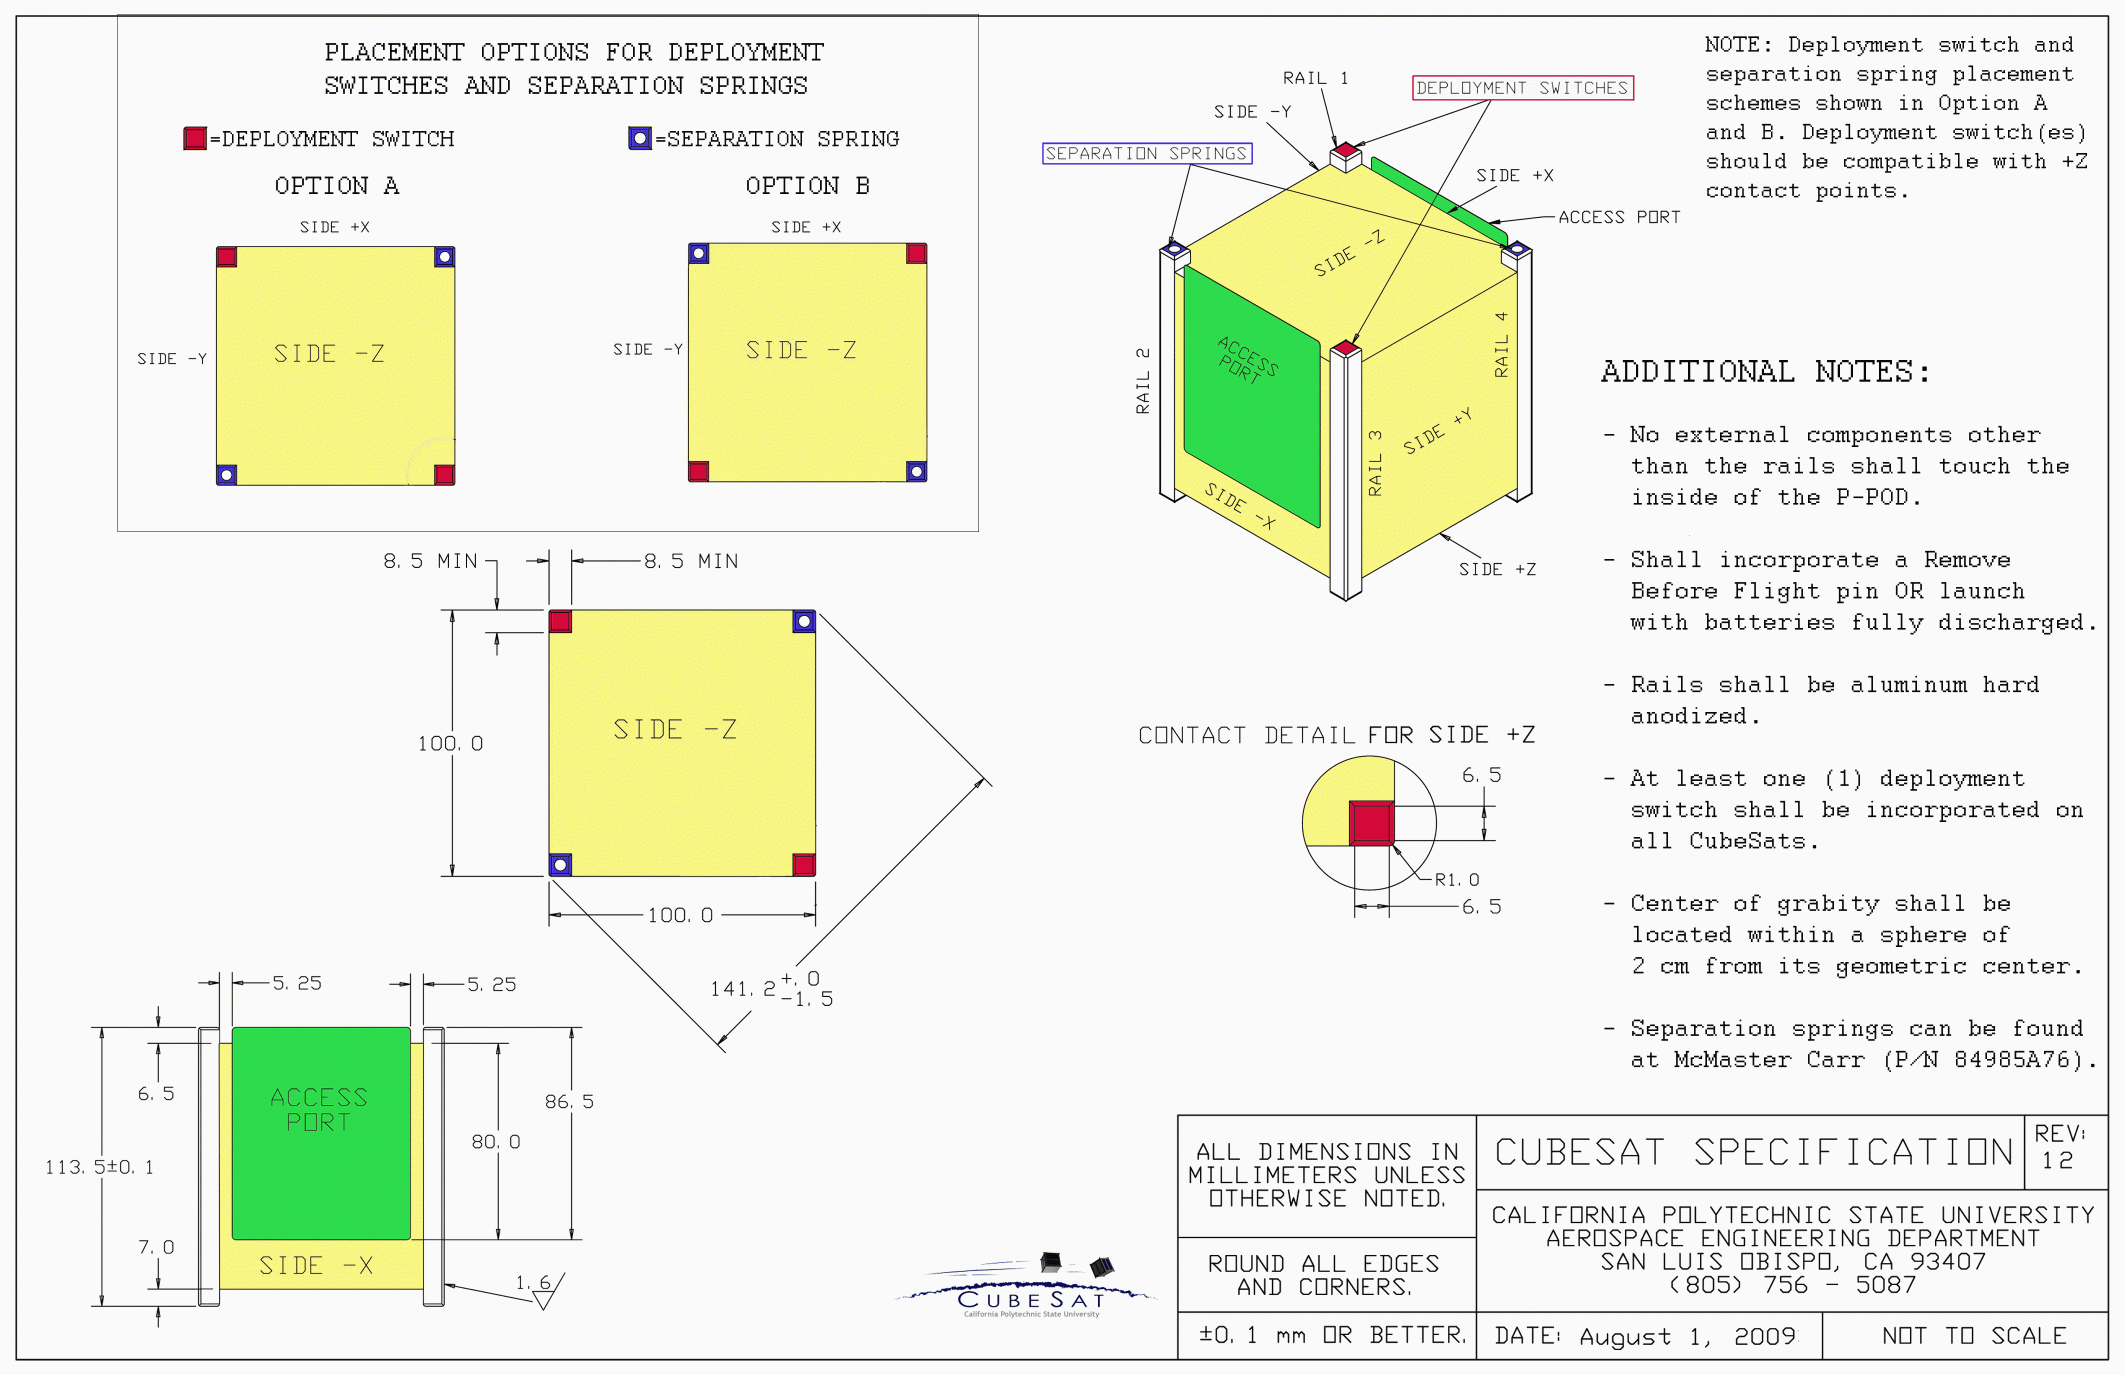
\includegraphics[scale=0.6]{./sections/SatelliteDesign/images/CubeSatDesign}
\centering
\caption{Dimensions of a 1U CubeSat \cite{cubesatdimensions}}
\end{figure}

\subsubsection{Structure}
EMPTY
\subsubsection{Deployments}
EMPTY
\subsubsection{Thermal protection}
\paragraph{}The thermal protection system protect the CubeSat from thermal shocks. The satellite must remain in a optimal range of temperatures,despite the external temperature. It consists of various insulating materials and thermal conductors in order to maintain it within acceptable temperatures.

\subsubsection{Study of the commercial available options}
EMPTY

\begin{longtable}{| l | r | r | }
\hline
\rowcolor[gray]{0.80}	\textbf{Brand and model} &  \textbf{Features and description}     & \textbf{Money (\euro)}   \\
\hline
\endfirsthead

\rowcolor[gray]{0.85} \textbf{Solar Panels} &  &  \\
	   ~Fabricant 1 & EMPTY & 2000000 \\
	   ~Chuscas 1 & EMPTY & 20000 \\
	   ~Truñaas 1 & EMPTY & 20000 \\
	   ~Cuescas 1 & EMPTY & 20000 \\
	\hline

\caption{Options studied}
\label{epsoptionstable}
\end{longtable}

Of all the options in \ref{epsoptionstable}, we have chosen the following options.
